\documentclass{beamer}
\usepackage[utf8]{inputenc}
\usepackage{graphicx}
\usepackage{xcolor}
\usepackage{listings}
\usepackage{tikz}
\usepackage{graphicx}

\graphicspath{ {./figs/} }
\usetikzlibrary{fit}

\hypersetup{
    colorlinks=true,
    urlcolor=cyan
}

\title{Bubbles}
\author{Filip Peterek}
\institute{V\v{S}B-TUO}
\date{May 2024}

\begin{document}

\frame{\titlepage}

\section{BubbleML}

\begin{frame}
    \frametitle{BubbleML}
    \begin{itemize}
        \item Dataset
        \item Water boiling
        \begin{itemize}
            \item Water is heated to 80 degrees or more
            \item Visible water vapor
        \end{itemize}
        \item Stationary water (pool) or water moving through a tube
        \item Dataset is generated using Flash-X simulator
        \item Dataset consists of velocity, bubbles, temperature, pressure
        \item Dataset was used e.g. to train optical flow models
        \item \href{https://arxiv.org/pdf/2307.14623}{Paper}
    \end{itemize}
\end{frame}

\begin{frame}
    \frametitle{Visualized BubbleML dataset}
    \begin{center}
        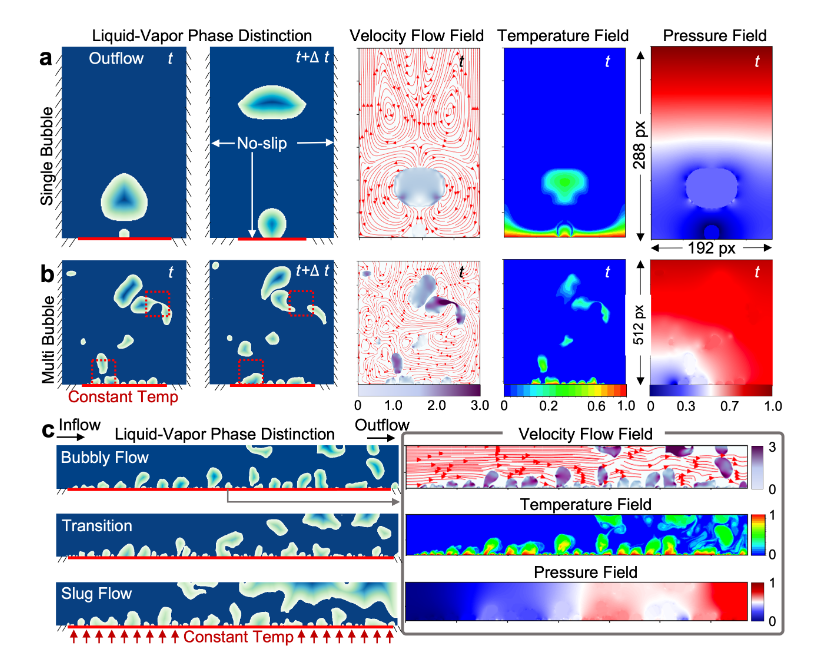
\includegraphics[width=0.8\columnwidth]{bubble-ml}
    \end{center}
    \href{https://arxiv.org/pdf/2307.14623}{Source}
\end{frame}

\section{Computational Fluid Dynamics}

\begin{frame}
    \frametitle{Computational Fluid Dynamics}
    \begin{itemize}
        \item Allows for generation of dataset
        \item Bubble movement can be simulated
        \item Plethora of paid and free solutions
        \item Very difficult to set up
    \end{itemize}
\end{frame}

\begin{frame}
    \frametitle{Computational Fluid Dynamics}
    \begin{itemize}
        \item \href{https://flash-x.org/}{Flash-X}
        \item \href{https://www.openfoam.com/}{OpenFOAM}
        \item \href{https://fluidsim.readthedocs.io/en/latest/}{Fluidsim}
        \item \href{https://www.cfdtool.com/}{CFD-Tool}
        \item \href{https://github.com/ProjectPhysX/FluidX3D}{FluidX3D}
        \item \href{https://github.com/unibas-dmi-hpc/SPH-EXA}{SPH-EXA}
        \item \href{https://www.sciencedirect.com/science/article/pii/S2352711020302922}{Lethe}
    \end{itemize}
\end{frame}

\begin{frame}
    \frametitle{Flash-X}
    \begin{itemize}
        \item Used to generate Bubble ML dataset
        \item Open source but requires registration via email to access
            \begin{itemize}
                \item Handled very quickly on maintainer side
            \end{itemize}
        \item Written in Fortran 90
        \item We had trouble building it
    \end{itemize}
\end{frame}

\begin{frame}
    \frametitle{OpenFOAM}
    \begin{itemize}
        \item Open source
        \item Written in C++
        \item Naval Hydro Pack can simulate open seas
        \item Bubble rising simulation
        \item Widely used, often recommended
        \item Custom configuration language
        \item Output is text files, one per simulation frame
        \item Python wrapper to setup simulations (PyFoamSetup)
        \item Seems like the best option when it comes to CFD
        \item Very difficult to learn
    \end{itemize}
\end{frame}

\begin{frame}
    \frametitle{Naval Hydro Pack}
    \begin{center}
        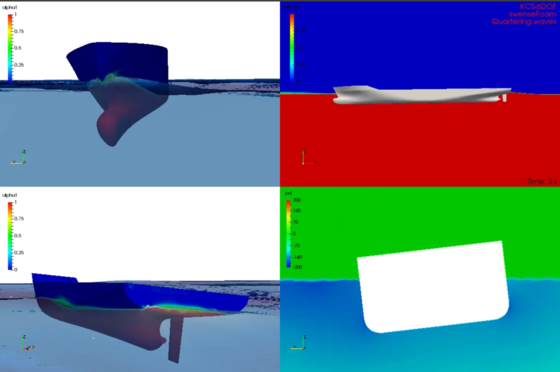
\includegraphics[width=0.8\columnwidth]{naval-hydro}
    \end{center}
    \href{https://openfoam-extend.sourceforge.net/OpenFOAM_Workshops/OFW11_2016_Guimaraes/special.html}{Source}
\end{frame}

\begin{frame}
    \frametitle{Bubble Rising}
    \begin{center}
        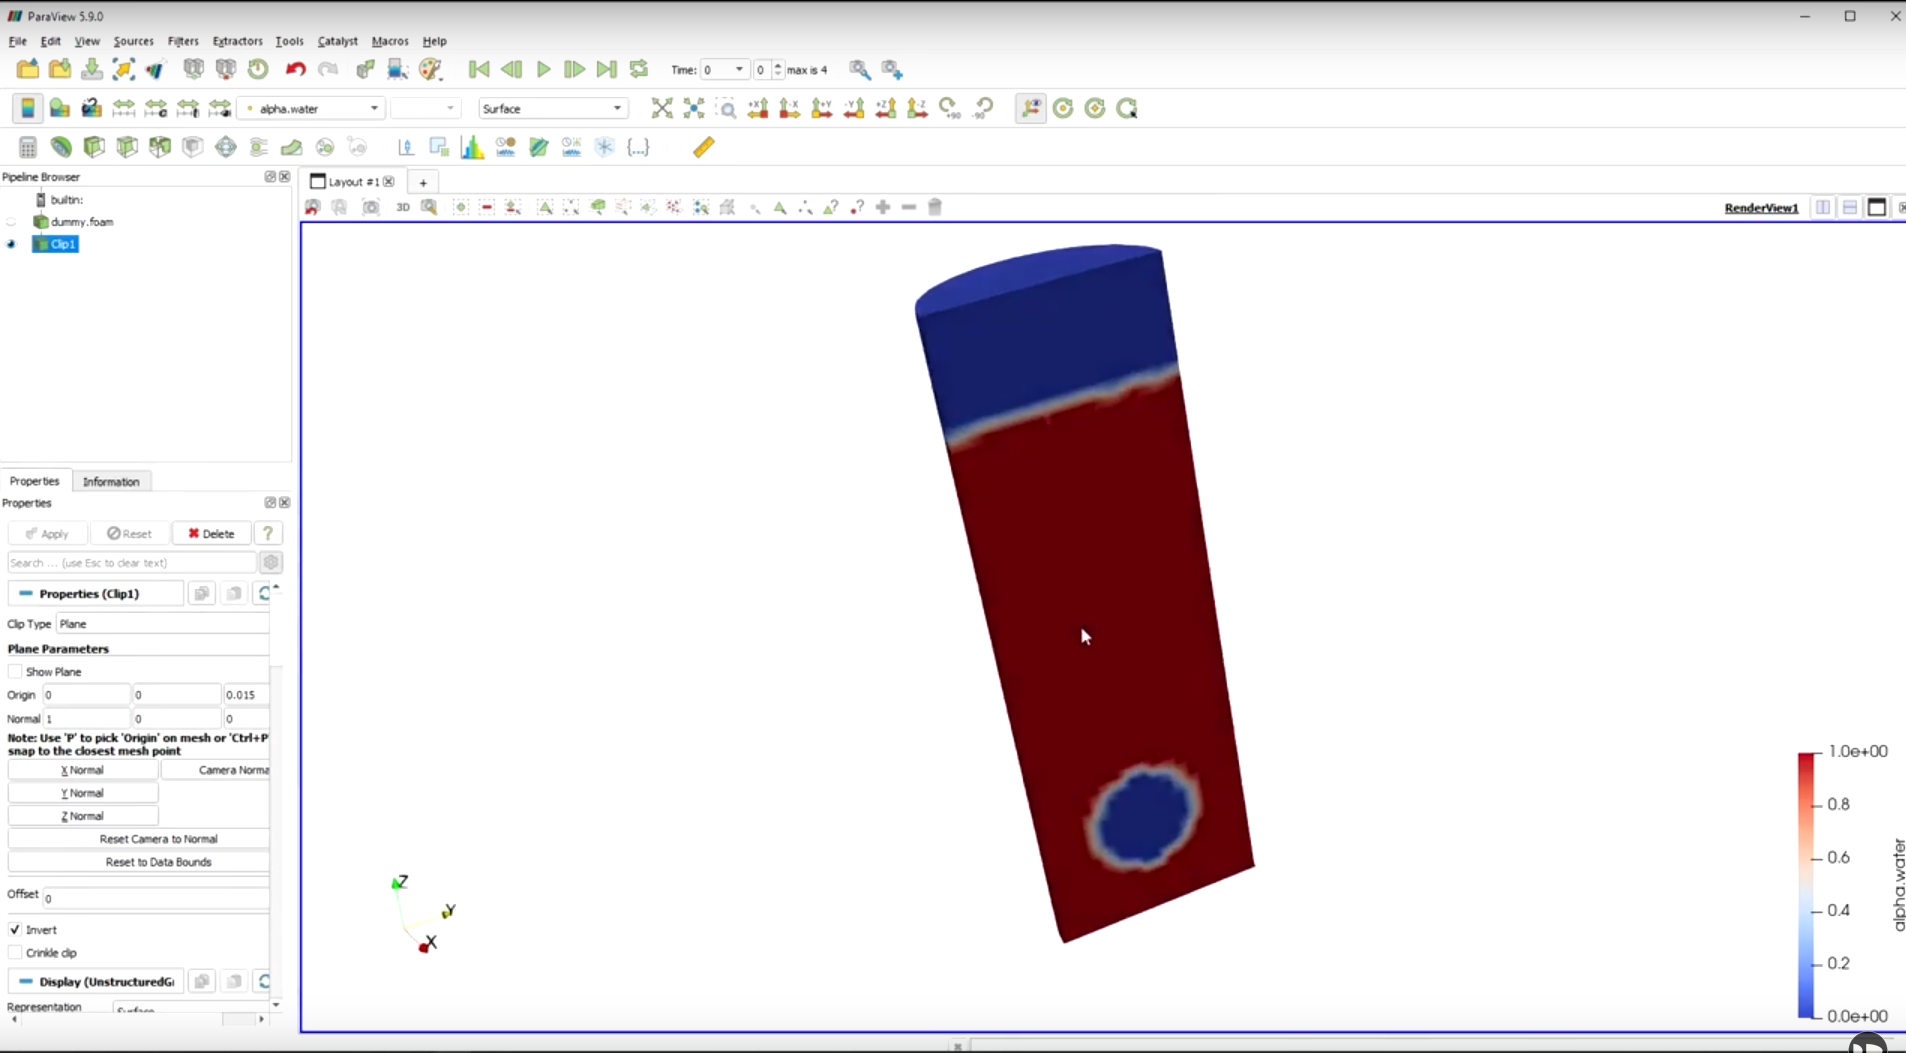
\includegraphics[width=0.8\columnwidth]{bubble-rising-1}
    \end{center}
    \href{https://www.youtube.com/watch?v=JYHhF25OTm0}{Source}
\end{frame}

\begin{frame}
    \frametitle{Bubble Rising}
    \begin{center}
        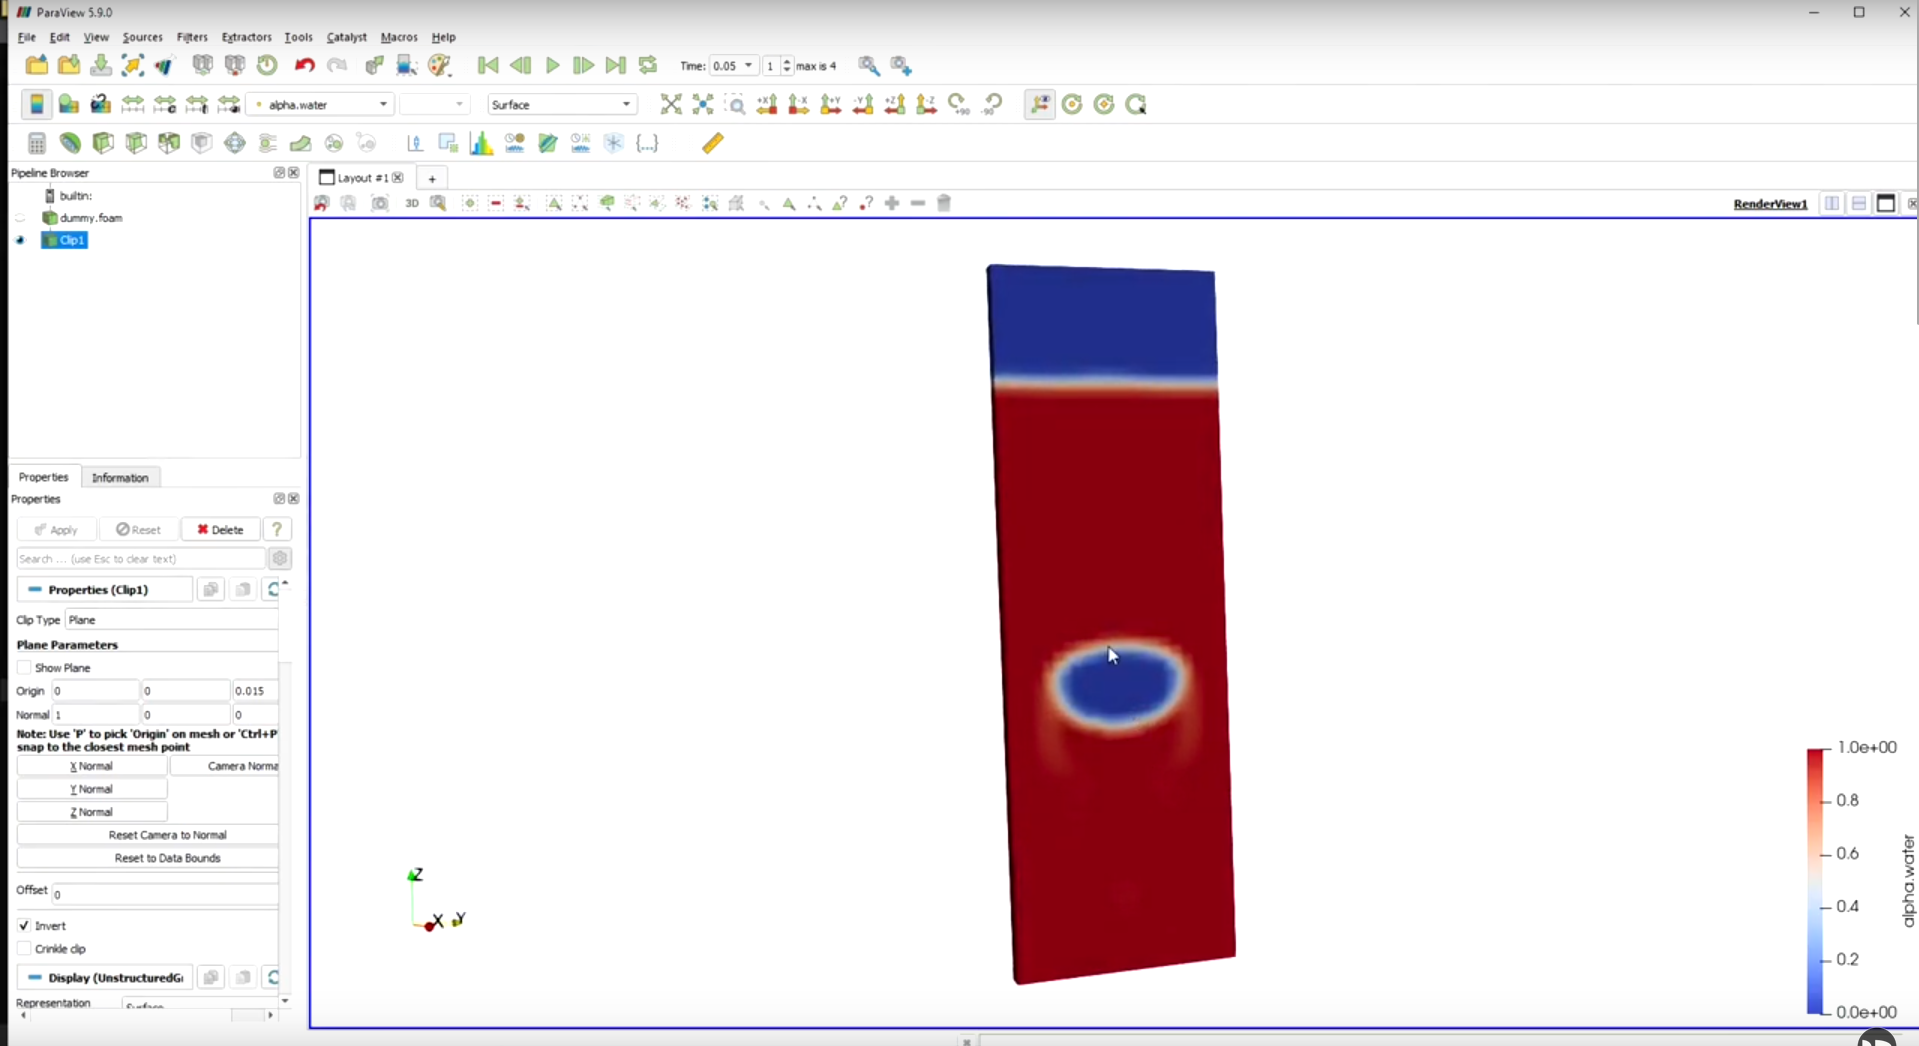
\includegraphics[width=0.8\columnwidth]{bubble-rising-2}
    \end{center}
    \href{www.youtube.com/watch?v=JYHhF25OTm0}{Source}
\end{frame}

\begin{frame}
    \frametitle{Bubble Rising}
    \begin{center}
        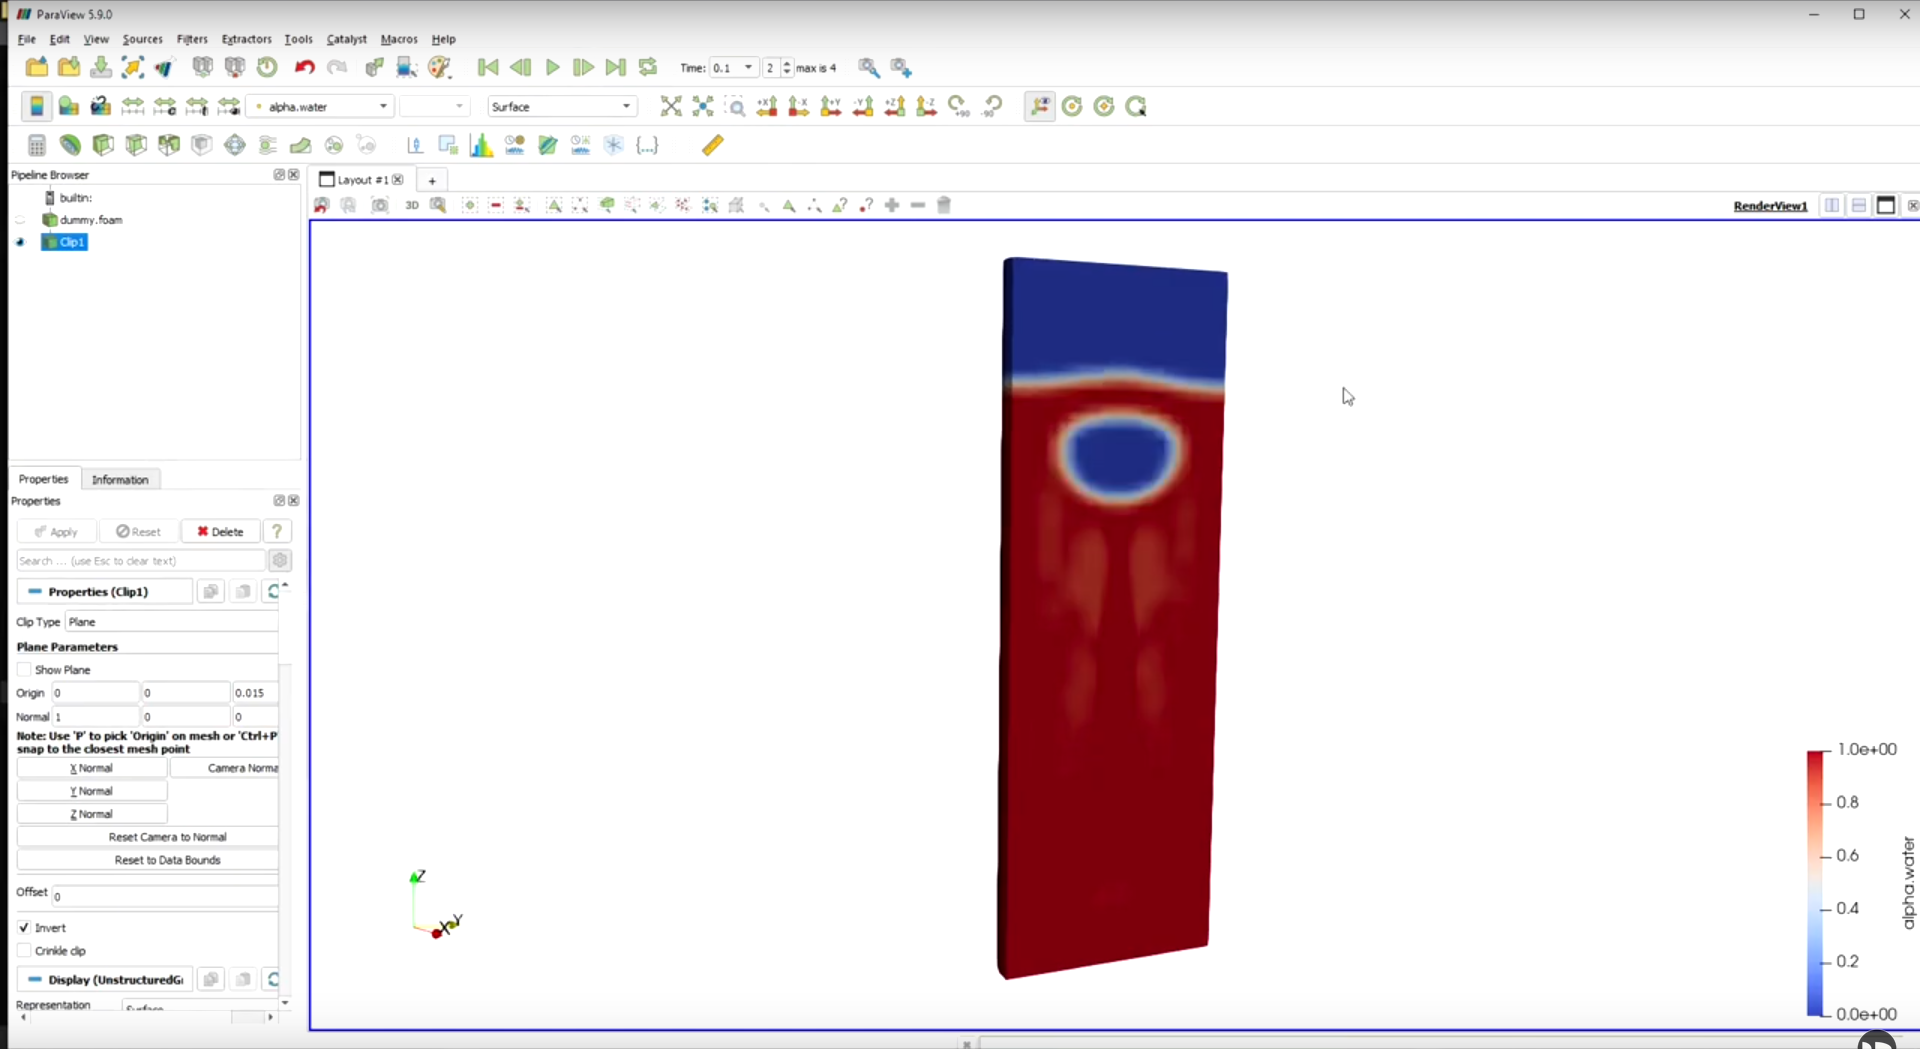
\includegraphics[width=0.8\columnwidth]{bubble-rising-3}
    \end{center}
    \href{www.youtube.com/watch?v=JYHhF25OTm0}{Source}
\end{frame}

\begin{frame}
    \frametitle{Bubble Rising}
    \begin{center}
        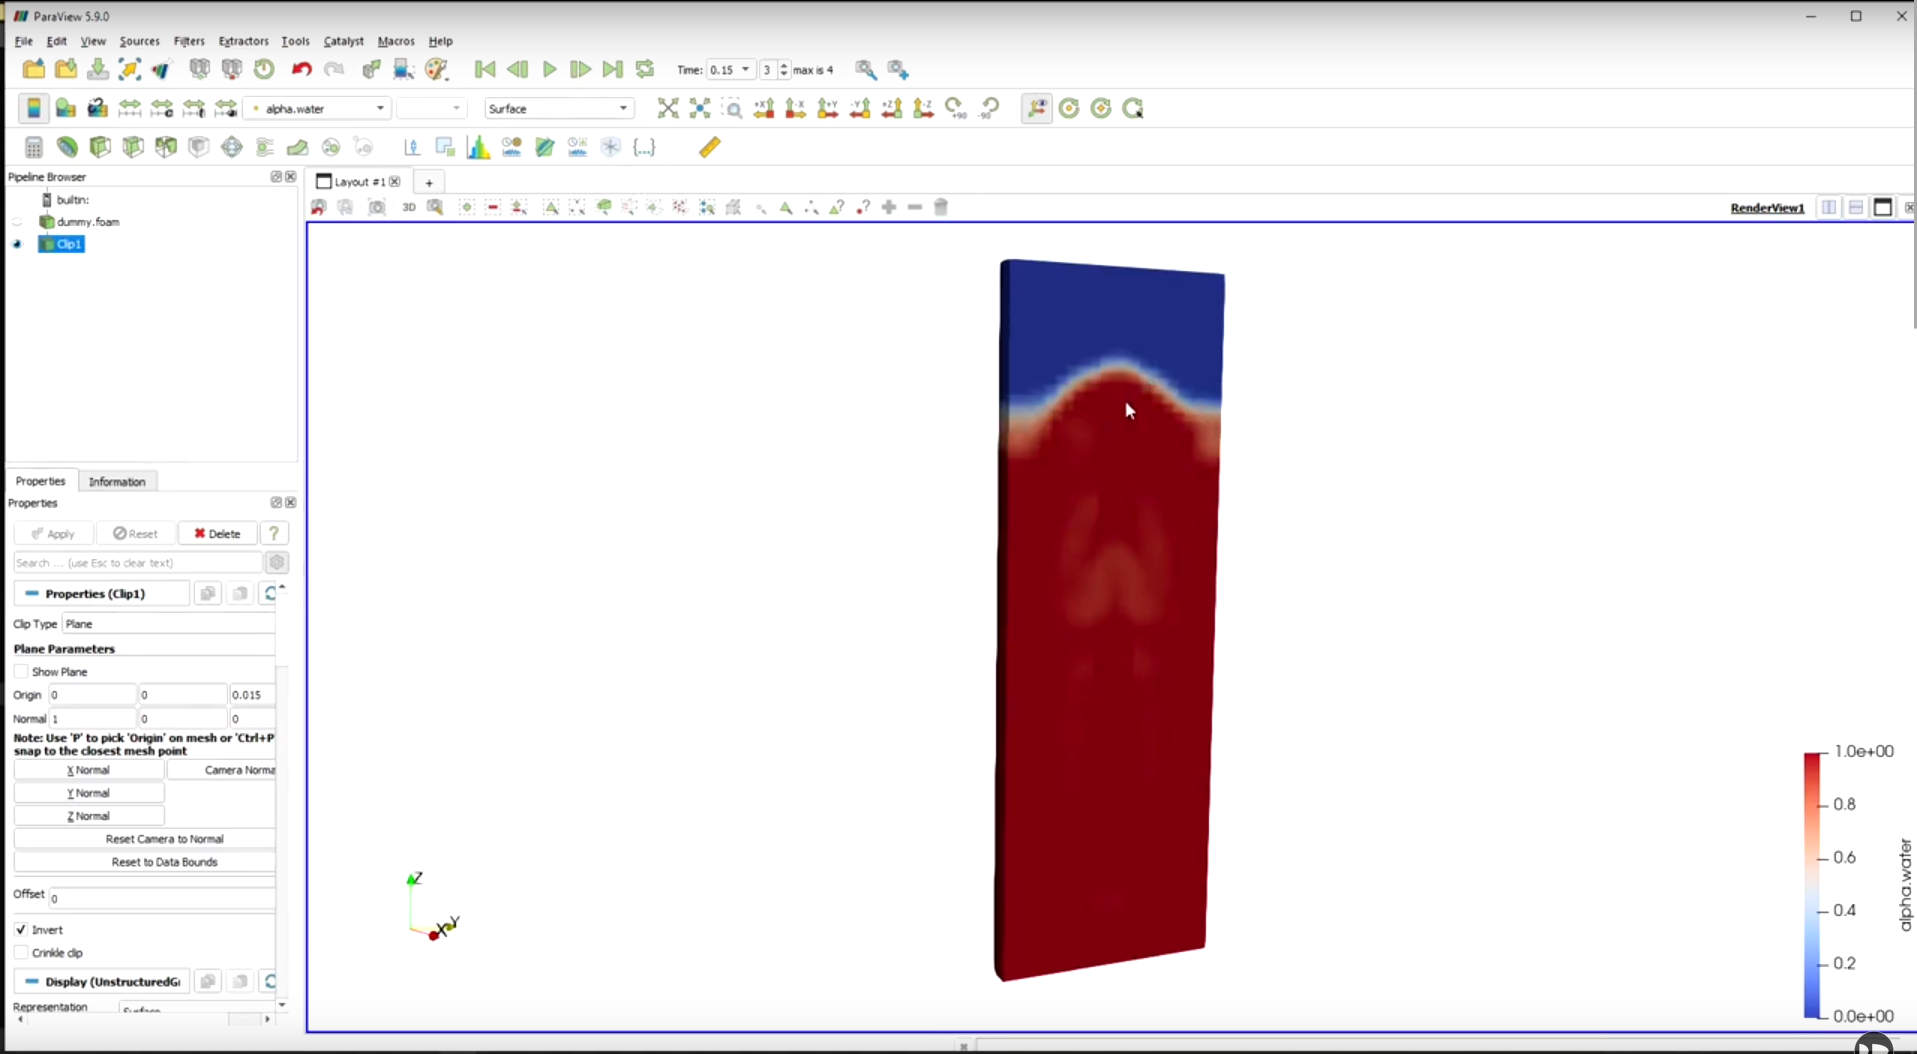
\includegraphics[width=0.8\columnwidth]{bubble-rising-4}
    \end{center}
    \href{www.youtube.com/watch?v=JYHhF25OTm0}{Source}
\end{frame}

\begin{frame}
    \frametitle{CFDTool}
    \begin{itemize}
        \item Matlab toolbox
        \item Commercial project
        \item Can use multiple CFD solvers
        \item Includes OpenFOAM integration
    \end{itemize}
\end{frame}

\begin{frame}
    \frametitle{CFDTool}
    \begin{center}
        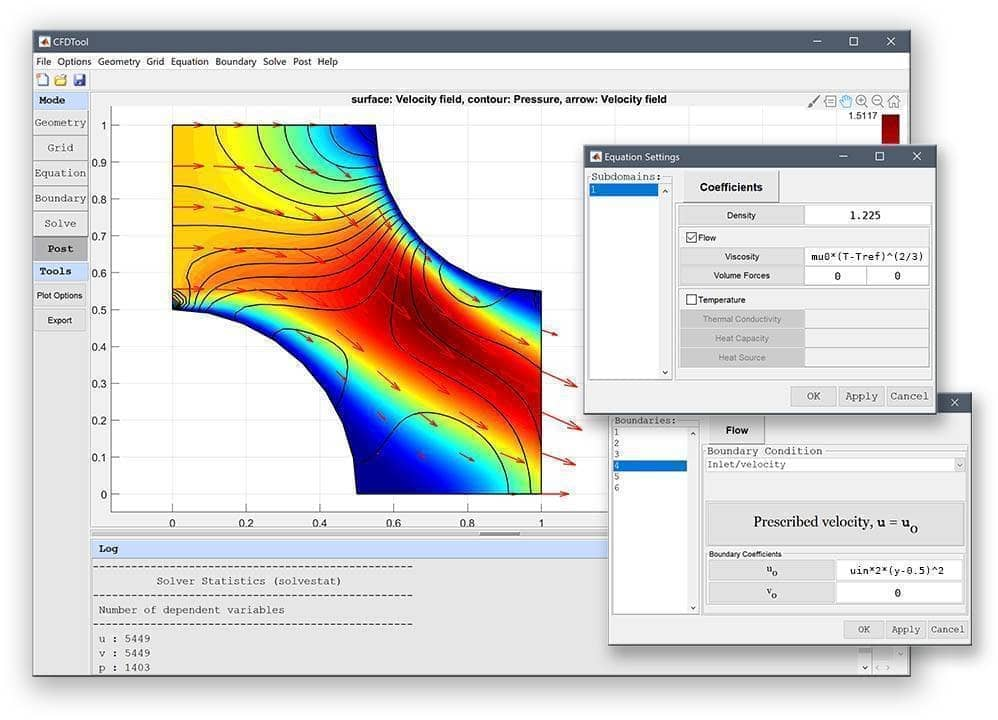
\includegraphics[width=0.8\columnwidth]{cfdtool}
    \end{center}
    \href{https://github.com/precise-simulation/cfdtool/tree/master}{Source}
\end{frame}



\section {Optical Models For Bubble Tracking}

\begin{frame}
    \frametitle{Bubble velocimetry using the conventional and CNN-based optical flow algorithms}
    \begin{itemize}
        \item Claims there are no suitable datasets
        \item Images in this paper are generated
            \begin{itemize}
                \item Bubbles move randomly
                \item May not change shape
            \end{itemize}
        \item CNNs used to detect bubbles
        \item Predicts bubble velocity
        \item CNN-based model (PWC-Net)
        \item Lucas-Kanade and Farnebäck methods
        \item \href{https://www.nature.com/articles/s41598-022-16145-y}{Paper}
    \end{itemize}
\end{frame}

\begin{frame}
    \frametitle{Deep learning-based automated and universal bubble detection and mask extraction in complex two-phase flows.}
    \begin{itemize}
        \item Referenced by the previous paper
        \item Promises to detect up to 95\% of all bubbles
        \item Detection software is FOSS and \href{https://github.com/ywflow/BubMask}{available on Github}
        \item \href{https://www.nature.com/articles/s41598-021-88334-0}{Paper}
    \end{itemize}
\end{frame}

\begin{frame}
    \frametitle{BubbleML}
    \begin{itemize}
        \item Model pretrained on flying chairs
        \item RAFT and GMFlow
        \item Suggest physics-informed models should be used
        \item Bubbles change shape and thus are difficult to track
        \item \href{https://github.com/HPCForge/BubbleML}{Github repository} contains examples of BubbleML usage
    \end{itemize}
\end{frame}

\end{document}
